\documentclass{beamer}

\beamertemplatenavigationsymbolsempty


\mode<presentation>
{
\usetheme[width=0cm]{Goettingen}
\usecolortheme{seahorse}
\useoutertheme{SEFM}
}

\input{header}
\usepackage[english]{babel}
% or whatever

\usepackage[utf8x]{inputenc}

\usepackage{times}
\usepackage[T1]{fontenc}


% Or whatever. Note that the encoding and the font should match. If T1
% does not look nice, try deleting the line with the fontenc.

\usepackage{pgf,tikz}
\usetikzlibrary{decorations}
\usetikzlibrary{shapes.arrows}
\usepackage{url}

%% Define a new 'leo' style for the package that will use a smaller font.
\makeatletter
\def\url@leostyle{%
  \def\UrlFont{\sf\small}}
\makeatother
%% Now actually use the newly defined style.
\urlstyle{leo}

\lstdefinelanguage{Smalltalk}{
  basicstyle=\ttfamily,
  keywordstyle=\bfseries,
  morekeywords={self,super,true,false,nil,thisContext}, % This is overkill
  morestring=[d]',
  morecomment=[s]{"}{"},
  alsoletter={\#:},
  escapechar={!},
}[keywords,comments,strings]


\newcommand{\Blue}[1]{\color{blue}#1\color{black}}

\title[OOP - OO Concepts and Smalltalk]{Object-Oriented
  Programming}

\subtitle[Concepts and Smalltalk]{OO Concepts and Smalltalk Introduction} %
%{OOP} % (optional)


\author[Richard Bubel] % (optional, use only with lots of authors)
{Richard Bubel \\ based on slides from Sibylle Schupp and Jean-Philippe Bernardy}
% - Use the \inst{?} command only if the authors have different
%   affiliation.

% - Use the \inst command only if there are several affiliations.
% - Keep it simple, no one is interested in your street address.

\institute[CTH]{Chalmers University of Technology}

\date{19th November 2010}%[Short Occasion] % (optional)


\subject{Talks}
% This is only inserted into the PDF information catalog. Can be left
% out.



% If you have a file called "university-logo-filename.xxx", where xxx
% is a graphic format that can be processed by latex or pdflatex,
% resp., then you can add a logo as follows:

%\pgfdeclareimage[height=0.5cm]{university-logo}{../../../project/gitroot/clipart/ChalmGUmarke.pdf}
% \logo{\pgfuseimage{university-logo}}


\begin{document}
\begin{frame}
  \titlepage
\end{frame}

\begin{frame}[fragile]
\frametitle{References}
References:
\begin{itemize}
\item M. Scott, Programming Language Pragmatics

\url{http://www.cs.rochester.edu/u/scott/254/notes/09-objects}
\item K. Loudon, Programming Languages---Principles and Practice
(not on-line available)
\end{itemize}

Additional reading:
\begin{itemize}
\item B. Ryders, Univ. Rutgers
\url{
http://remus.rutgers.edu/cs314/s2004/ryder/lectures/adt-15Newest-2up.pdf
}
%
\item K. Bruce, Williams College
\url{
http://www.cs.williams.edu/~kim/cs334/s00/Lectures/Lec13/Lec13.html}
\end{itemize}
\end{frame}

\mycomment {
\begin{frame}[fragile]
\frametitle{Premier (academic) conferences}
\framesubtitle{}

OOPSLA
\begin{itemize}
\item Object-Oriented Programming, Systems, Languages, and Applications
\item 2007: 21th Conference (ACM)
\item \url{http://www.oopsla.org}
\end{itemize}

ECOOP
\begin{itemize}
\item European Conference on Object-Oriented Programming
\item 2007: 22nd Conference (ACM)
\item \url{http://www.ecoop.org}
\end{itemize}

Turing award
\begin{itemize}
\item Ole-Johan Dahl, Kristen Nygaard (Simula), 2001
\item Alan Kay (Smalltalk), 2003
\end{itemize}
\end{frame}
}


\begin{frame}[fragile]
\frametitle{A short history}
%Scott, p.788
First generation
\begin{itemize}
\item SIMULA1 (1962), SIMULA 67 (1967): 
\begin{itemize}
\item Ole-Johan Dahl, Kristen Nygaard, Oslo
\item Inheritance, virtual methods
\end{itemize}
\item Smalltalk (1969) 
\begin{itemize}
\item Alan Kay, Dan Ingalls, Adele Goldberg at Xerox Parc
\item Dynamic language %(dynamic typing)
\end{itemize}
\end{itemize}

80s
\begin{itemize}
\item \cpp(1983)
%\begin{itemize}
%\item 
B. Stroustrup, AT\&T; hybrid
%\end{itemize}
\item Eiffel (1986); B. Meyer, ISI; %design by contract

\end{itemize}

And later many more:
\begin{itemize}
\item BETA, SELF, Ruby, \ldots
\item Modula-3, Oberon, Ada95, Sather, \ldots
\item Objective CAML, Objective-C, \ldots
\item Java (1995), C\# (2000)


\end{itemize}

\end{frame}



\section{OOP Basics}
\begin{frame}[fragile]
\frametitle{Structured Data}
\Blue{Built-in types:}\ integers, characters, etc.

\bigskip

\Blue{Need to represent \emph{user-defined} complex data?}\\
E.g., contact card in an address book

\bigskip

\Blue{Solution:}\ Structured data: records/structs 

A record defines a new type grouping a collection of attributes:

\begin{cplus3}
struct Person {
   char *name;
   int birthyear;
};
\end{cplus3}

defines a new type called \texttt{struct Person}.

Programming languages supporting records/structs must
\begin{itemize}
\item provide selectors for the components
\item means of creating a new record
\item copy semantics vs. reference semantics; shallow vs. deep-copy
\end{itemize}
\end{frame}


\begin{frame}[fragile]
\frametitle{Structured Data - Cont'd}

Usage of records:
\begin{itemize}
  \item<+-> Records globally known? Can any procedure operate on it? 
  \item<+-> Specialisation/Extension of records? How?
  \item<+-> How to deal with structural changes of a record?
\end{itemize}

\onslide<+->\bigskip\bigskip

Starting point for the introduction of \emph{classes} and
\emph{objects}:\\
\begin{center}
  Group records and operations on records
\end{center}

\end{frame}



\begin{frame}[fragile]
\frametitle{What are objects?}
\framesubtitle{}

\emph{Objects} are entities with 
\begin{itemize}
  \item a \emph{modifiable state} and 
  \item a set of \emph{functions} to access and change that state
\end{itemize}

\pause\medskip

Modifiable state 
\begin{itemize}
  \item ideally local (private) to object (\emph{data encapsulation})
  \item local object variables are called \emph{fields} or
    \emph{instance variables} 
\end{itemize}

\pause\medskip

\emph{Functions} in OOP
\begin{itemize}
\item are called \textit{methods} or \textit{messages}.
\item have an implicit parameter, the object itself (``this'', ``self'').
\end{itemize}

\pause\medskip

An object \textit{instantiates} a class.
\end{frame}

\begin{frame}[fragile]
\frametitle{What are classes?}
\framesubtitle{}

A \emph{class} is a blueprint (construction scheme) for objects.

\bigskip

A class

\begin{itemize}
\item groups the fields and methods of an object.
\item is \textit{instantiable} by objects.
It contains \textit{constructors} to allocate and initialize objects.
\item is a unit of inheritance: it is derived from another
class and one can use it to derive a new class from it. 
\item is a type. 
% in statically-typed languages
\end{itemize}
\bigskip
Most OO-languages permit classes that do not (have to) exhibit all aspects. 
\end{frame}


\begin{frame}[fragile]
\frametitle{Object Model}
\begin{minipage}{0.64\textwidth}
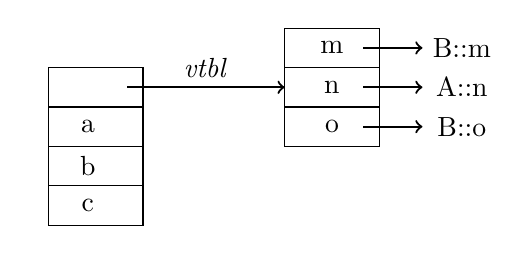
\begin{tikzpicture}

\draw (0,-2.0)  rectangle (1.2,-1.0);
\draw (0,-1.0)  rectangle (1.2,-1.5);
\draw (0,-1.5)  rectangle (1.2,-2.0);
\draw (0,-2.0)  rectangle (1.2,-2.5);
\pgftext[at={\pgfpoint{0.5cm}{-1.25cm}}]{a};
\pgftext[at={\pgfpoint{0.5cm}{-1.75cm}}]{b};
\pgftext[at={\pgfpoint{0.5cm}{-2.25cm}}]{c};

% vptr
\draw (0,-1.0)  rectangle (1.2,-0.5);
\pgftext[at={\pgfpoint{-0.25cm}{-0.75cm}}]{} ;
\draw[->, thick] (1.0, -0.75) -- (3.0,-0.75); 
\pgftext[at={\pgfpoint{2.0cm}{-0.5cm}}]{\textit{vtbl}} ;

% 
\draw (3.0,0) rectangle (4.2,-0.5);
\pgftext[at={\pgfpoint{3.6cm}{-0.25cm}}]{m} ;
\draw[->, thick] (4.0, -0.25) -- (4.75,-0.25); 
\pgftext[at={\pgfpoint{5.25cm}{-0.25cm}}]{B::m} ;

\draw (3.0,-0.5) rectangle (4.2,-1);
\pgftext[at={\pgfpoint{3.6cm}{-0.75cm}}]{n} ;
\draw[->, thick] (4.0, -0.75) -- (4.75,-0.75); 
\pgftext[at={\pgfpoint{5.25cm}{-0.75cm}}]{A::n} ;


\draw (3.0,-1) rectangle (4.2,-1.5);
\pgftext[at={\pgfpoint{3.6cm}{-1.25cm}}]{o} ;
\draw[->, thick] (4.0, -1.25) -- (4.75,-1.25); 
\pgftext[at={\pgfpoint{5.25cm}{-1.25cm}}]{B::o} ;

\end{tikzpicture}
\end{minipage}
\begin{minipage}{0.35\textwidth}
% Graphic for TeX using PGF
% Title: /Users/bubel/Documents/Teaching/Lectures/PP/prgprd/Lectures/objmodel.dia
% Creator: Dia v0.97.1
% CreationDate: Fri Nov 19 11:05:10 2010
% For: bubel
% \usepackage{tikz}
% The following commands are not supported in PSTricks at present
% We define them conditionally, so when they are implemented,
% this pgf file will use them.
\ifx\du\undefined
  \newlength{\du}
\fi
\setlength{\du}{15\unitlength}
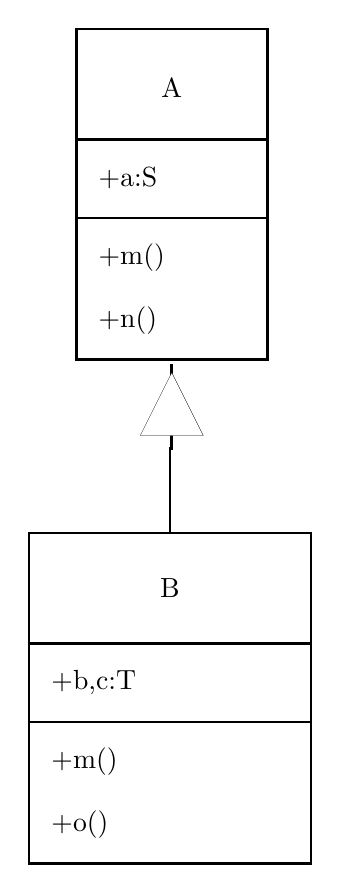
\begin{tikzpicture}
\pgftransformxscale{1.000000}
\pgftransformyscale{-1.000000}
\definecolor{dialinecolor}{rgb}{0.000000, 0.000000, 0.000000}
\pgfsetstrokecolor{dialinecolor}
\definecolor{dialinecolor}{rgb}{1.000000, 1.000000, 1.000000}
\pgfsetfillcolor{dialinecolor}
\pgfsetlinewidth{1pt}
\pgfsetdash{}{0pt}
\definecolor{dialinecolor}{rgb}{1.000000, 1.000000, 1.000000}
\pgfsetfillcolor{dialinecolor}
\fill (14.300000\du,5.900000\du)--(14.300000\du,7.300000\du)--(16.725000\du,7.300000\du)--(16.725000\du,5.900000\du)--cycle;
\definecolor{dialinecolor}{rgb}{0.000000, 0.000000, 0.000000}
\pgfsetstrokecolor{dialinecolor}
\draw (14.300000\du,5.900000\du)--(14.300000\du,7.300000\du)--(16.725000\du,7.300000\du)--(16.725000\du,5.900000\du)--cycle;
% setfont left to latex
\definecolor{dialinecolor}{rgb}{0.000000, 0.000000, 0.000000}
\pgfsetstrokecolor{dialinecolor}
\node at (15.512500\du,6.650000\du){A};
\definecolor{dialinecolor}{rgb}{1.000000, 1.000000, 1.000000}
\pgfsetfillcolor{dialinecolor}
\fill (14.300000\du,7.300000\du)--(14.300000\du,8.300000\du)--(16.725000\du,8.300000\du)--(16.725000\du,7.300000\du)--cycle;
\definecolor{dialinecolor}{rgb}{0.000000, 0.000000, 0.000000}
\pgfsetstrokecolor{dialinecolor}
\draw (14.300000\du,7.300000\du)--(14.300000\du,8.300000\du)--(16.725000\du,8.300000\du)--(16.725000\du,7.300000\du)--cycle;
% setfont left to latex
\definecolor{dialinecolor}{rgb}{0.000000, 0.000000, 0.000000}
\pgfsetstrokecolor{dialinecolor}
\node[anchor=west] at (14.450000\du,7.8000000\du){+a:S};
\definecolor{dialinecolor}{rgb}{1.000000, 1.000000, 1.000000}
\pgfsetfillcolor{dialinecolor}
\fill (14.300000\du,8.300000\du)--(14.300000\du,10.100000\du)--(16.725000\du,10.100000\du)--(16.725000\du,8.300000\du)--cycle;
\definecolor{dialinecolor}{rgb}{0.000000, 0.000000, 0.000000}
\pgfsetstrokecolor{dialinecolor}
\draw (14.300000\du,8.300000\du)--(14.300000\du,10.100000\du)--(16.725000\du,10.100000\du)--(16.725000\du,8.300000\du)--cycle;
% setfont left to latex
\definecolor{dialinecolor}{rgb}{0.000000, 0.000000, 0.000000}
\pgfsetstrokecolor{dialinecolor}
\node[anchor=west] at (14.450000\du,8.800000\du){+m()};
% setfont left to latex
\definecolor{dialinecolor}{rgb}{0.000000, 0.000000, 0.000000}
\pgfsetstrokecolor{dialinecolor}
\node[anchor=west] at (14.450000\du,9.600000\du){+n()};
\pgfsetlinewidth{1pt}
\pgfsetdash{}{0pt}
\definecolor{dialinecolor}{rgb}{1.000000, 1.000000, 1.000000}
\pgfsetfillcolor{dialinecolor}
\fill (13.700000\du,12.300000\du)--(13.700000\du,13.700000\du)--(17.280000\du,13.700000\du)--(17.280000\du,12.300000\du)--cycle;
\definecolor{dialinecolor}{rgb}{0.000000, 0.000000, 0.000000}
\pgfsetstrokecolor{dialinecolor}
\draw (13.700000\du,12.300000\du)--(13.700000\du,13.700000\du)--(17.280000\du,13.700000\du)--(17.280000\du,12.300000\du)--cycle;
% setfont left to latex
\definecolor{dialinecolor}{rgb}{0.000000, 0.000000, 0.000000}
\pgfsetstrokecolor{dialinecolor}
\node at (15.490000\du,13.0000\du){B};
\definecolor{dialinecolor}{rgb}{1.000000, 1.000000, 1.000000}
\pgfsetfillcolor{dialinecolor}
\fill (13.700000\du,13.700000\du)--(13.700000\du,14.700000\du)--(17.280000\du,14.700000\du)--(17.280000\du,13.700000\du)--cycle;
\definecolor{dialinecolor}{rgb}{0.000000, 0.000000, 0.000000}
\pgfsetstrokecolor{dialinecolor}
\draw (13.700000\du,13.700000\du)--(13.700000\du,14.700000\du)--(17.280000\du,14.700000\du)--(17.280000\du,13.700000\du)--cycle;
% setfont left to latex
\definecolor{dialinecolor}{rgb}{0.000000, 0.000000, 0.000000}
\pgfsetstrokecolor{dialinecolor}
\node[anchor=west] at (13.850000\du,14.200000\du){+b,c:T};
\definecolor{dialinecolor}{rgb}{1.000000, 1.000000, 1.000000}
\pgfsetfillcolor{dialinecolor}
\fill (13.700000\du,14.700000\du)--(13.700000\du,16.500000\du)--(17.280000\du,16.500000\du)--(17.280000\du,14.700000\du)--cycle;
\definecolor{dialinecolor}{rgb}{0.000000, 0.000000, 0.000000}
\pgfsetstrokecolor{dialinecolor}
\draw (13.700000\du,14.700000\du)--(13.700000\du,16.500000\du)--(17.280000\du,16.500000\du)--(17.280000\du,14.700000\du)--cycle;
% setfont left to latex
\definecolor{dialinecolor}{rgb}{0.000000, 0.000000, 0.000000}
\pgfsetstrokecolor{dialinecolor}
\node[anchor=west] at (13.850000\du,15.200000\du){+m()};
% setfont left to latex
\definecolor{dialinecolor}{rgb}{0.000000, 0.000000, 0.000000}
\pgfsetstrokecolor{dialinecolor}
\node[anchor=west] at (13.850000\du,16.000000\du){+o()};
\pgfsetlinewidth{1pt}
\pgfsetdash{}{0pt}
\pgfsetmiterjoin
\pgfsetbuttcap
{
\definecolor{dialinecolor}{rgb}{0.000000, 0.000000, 0.000000}
\pgfsetfillcolor{dialinecolor}
% was here!!!
\definecolor{dialinecolor}{rgb}{0.000000, 0.000000, 0.000000}
\pgfsetstrokecolor{dialinecolor}
\draw (15.512500\du,10.150262\du)--(15.512500\du,11.225131\du)--(15.490000\du,11.225131\du)--(15.490000\du,12.300000\du);
}
\definecolor{dialinecolor}{rgb}{0.000000, 0.000000, 0.000000}
\pgfsetstrokecolor{dialinecolor}
\draw (15.512500\du,11.062066\du)--(15.512500\du,11.225131\du)--(15.490000\du,11.225131\du)--(15.490000\du,12.300000\du);
\pgfsetmiterjoin
\definecolor{dialinecolor}{rgb}{1.000000, 1.000000, 1.000000}
\pgfsetfillcolor{dialinecolor}
\fill (15.912500\du,11.062066\du)--(15.512500\du,10.262066\du)--(15.112500\du,11.062066\du)--cycle;
\pgfsetlinewidth{0.100000\du}
\pgfsetdash{}{0pt}
\pgfsetmiterjoin
\definecolor{dialinecolor}{rgb}{0.000000, 0.000000, 0.000000}
\pgfsetstrokecolor{dialinecolor}
\draw (15.912500\du,11.062066\du)--(15.512500\du,10.262066\du)--(15.112500\du,11.062066\du)--cycle;
% setfont left to latex
\end{tikzpicture}

\end{minipage}
\bigskip

vtbl: virtual method table

\end{frame}



\subsubsection{Methods}
\begin{frame}[fragile]
\frametitle{Methods}
\framesubtitle{}
If we ignore inheritance (for the moment), class methods  are
quite similar to top-level functions. 
\bigskip

Difference:
\begin{itemize}
\item Implicit ``this'' parameter: receiver object 
\begin{itemize}
\begin{cplus3}
// free function 'add'
complex add(const complex& x, const complex& y) {...}

// method 'add'
class complex {
    complex add(const complex& y) {...}
};
\end{cplus3}
\item Exception: static methods
\end{itemize}
\item Can access the internal state.
\end{itemize}
\end{frame}

\begin{frame}[fragile]
\frametitle{Constructors and initialization}
Object creation is typically done by constructors. Two tasks:
\begin{itemize}
\item Allocate memory 
\item Initialize fields

\end{itemize}
\framesubtitle{}
%se.ethz.ch/teaching/ss2006/0050/slides/eiffel_the_essentials.pdf 
\bigskip

Syntax (example) of constructor:
\begin{center}
\begin{lstlisting}[language=Java, basicstyle=\small\ttfamily, commentstyle=\scriptsize]
public class Point {
  ...
  public Point(int x, int y) {
     this.x = x; this.y = y;
  } 
}
// invoked via
Point p = new Point(10,10);
\end{lstlisting}
\end{center}
Other languages:
\begin{itemize}
\item Modula-3 provides no constructors
\item Ada95 only for objects derived from Controlled
\item \Cpp/Java have default constructors (initialization not required).
\end{itemize}
\end{frame}


\subsection{Inheritance}



\begin{frame}[fragile]
\frametitle{Inheritance}
\framesubtitle{}

\begin{center}
  A subclass is an \emph{extension} of its \emph{superclass}.
\end{center}

\bigskip

Syntax (examples)

\begin{cplus3}
   '' Smalltalk''
    Shape subclass: #Rectangle
        instanceVariableNames: 'width height'
        classVariableNames: ''
        poolDictionaries: ''
        category: ''

     // C# and C++
     public class Rectangle: Shape {
        ... 
     }
\end{cplus3}


\end{frame}


\begin{frame}[fragile]
\frametitle{Example}
\framesubtitle{}
\bigskip

\begin{center}
\begin{minipage}{0.3\textwidth}
% Graphic for TeX using PGF
% Title: /Users/bubel/Documents/Teaching/Lectures/PP/prgprd/Lectures/objmodel2.dia
% Creator: Dia v0.97.1
% CreationDate: Fri Nov 19 11:16:55 2010
% For: bubel
% \usepackage{tikz}
% The following commands are not supported in PSTricks at present
% We define them conditionally, so when they are implemented,
% this pgf file will use them.
\ifx\du\undefined
  \newlength{\du}
\fi
\setlength{\du}{14\unitlength}
\small
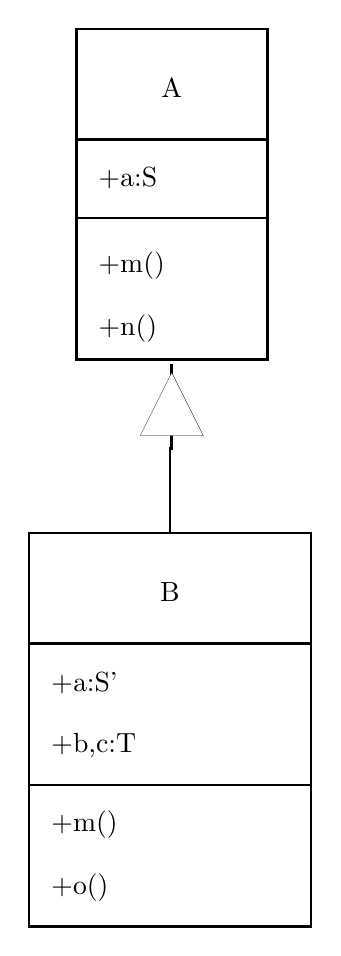
\begin{tikzpicture}
\pgftransformxscale{1.000000}
\pgftransformyscale{-1.000000}
\definecolor{dialinecolor}{rgb}{0.000000, 0.000000, 0.000000}
\pgfsetstrokecolor{dialinecolor}
\definecolor{dialinecolor}{rgb}{1.000000, 1.000000, 1.000000}
\pgfsetfillcolor{dialinecolor}
\pgfsetlinewidth{1pt}
\pgfsetdash{}{0pt}
\definecolor{dialinecolor}{rgb}{1.000000, 1.000000, 1.000000}
\pgfsetfillcolor{dialinecolor}
\fill (14.300000\du,5.900000\du)--(14.300000\du,7.300000\du)--(16.725000\du,7.300000\du)--(16.725000\du,5.900000\du)--cycle;
\definecolor{dialinecolor}{rgb}{0.000000, 0.000000, 0.000000}
\pgfsetstrokecolor{dialinecolor}
\draw (14.300000\du,5.900000\du)--(14.300000\du,7.300000\du)--(16.725000\du,7.300000\du)--(16.725000\du,5.900000\du)--cycle;
% setfont left to latex
\definecolor{dialinecolor}{rgb}{0.000000, 0.000000, 0.000000}
\pgfsetstrokecolor{dialinecolor}
\node at (15.512500\du,6.650000\du){A};
\definecolor{dialinecolor}{rgb}{1.000000, 1.000000, 1.000000}
\pgfsetfillcolor{dialinecolor}
\fill (14.300000\du,7.300000\du)--(14.300000\du,8.300000\du)--(16.725000\du,8.300000\du)--(16.725000\du,7.300000\du)--cycle;
\definecolor{dialinecolor}{rgb}{0.000000, 0.000000, 0.000000}
\pgfsetstrokecolor{dialinecolor}
\draw (14.300000\du,7.300000\du)--(14.300000\du,8.300000\du)--(16.725000\du,8.300000\du)--(16.725000\du,7.300000\du)--cycle;
% setfont left to latex
\definecolor{dialinecolor}{rgb}{0.000000, 0.000000, 0.000000}
\pgfsetstrokecolor{dialinecolor}
\node[anchor=west] at (14.450000\du,7.800000\du){+a:S};
\definecolor{dialinecolor}{rgb}{1.000000, 1.000000, 1.000000}
\pgfsetfillcolor{dialinecolor}
\fill (14.300000\du,8.300000\du)--(14.300000\du,10.100000\du)--(16.725000\du,10.100000\du)--(16.725000\du,8.300000\du)--cycle;
\definecolor{dialinecolor}{rgb}{0.000000, 0.000000, 0.000000}
\pgfsetstrokecolor{dialinecolor}
\draw (14.300000\du,8.300000\du)--(14.300000\du,10.100000\du)--(16.725000\du,10.100000\du)--(16.725000\du,8.300000\du)--cycle;
% setfont left to latex
\definecolor{dialinecolor}{rgb}{0.000000, 0.000000, 0.000000}
\pgfsetstrokecolor{dialinecolor}
\node[anchor=west] at (14.450000\du,8.900000\du){+m()};
% setfont left to latex
\definecolor{dialinecolor}{rgb}{0.000000, 0.000000, 0.000000}
\pgfsetstrokecolor{dialinecolor}
\node[anchor=west] at (14.450000\du,9.700000\du){+n()};
\pgfsetlinewidth{1pt}
\pgfsetdash{}{0pt}
\definecolor{dialinecolor}{rgb}{1.000000, 1.000000, 1.000000}
\pgfsetfillcolor{dialinecolor}
\fill (13.700000\du,12.300000\du)--(13.700000\du,13.700000\du)--(17.280000\du,13.700000\du)--(17.280000\du,12.300000\du)--cycle;
\definecolor{dialinecolor}{rgb}{0.000000, 0.000000, 0.000000}
\pgfsetstrokecolor{dialinecolor}
\draw (13.700000\du,12.300000\du)--(13.700000\du,13.700000\du)--(17.280000\du,13.700000\du)--(17.280000\du,12.300000\du)--cycle;
% setfont left to latex
\definecolor{dialinecolor}{rgb}{0.000000, 0.000000, 0.000000}
\pgfsetstrokecolor{dialinecolor}
\node at (15.490000\du,13.050000\du){B};
\definecolor{dialinecolor}{rgb}{1.000000, 1.000000, 1.000000}
\pgfsetfillcolor{dialinecolor}
\fill (13.700000\du,13.700000\du)--(13.700000\du,15.500000\du)--(17.280000\du,15.500000\du)--(17.280000\du,13.700000\du)--cycle;
\definecolor{dialinecolor}{rgb}{0.000000, 0.000000, 0.000000}
\pgfsetstrokecolor{dialinecolor}
\draw (13.700000\du,13.700000\du)--(13.700000\du,15.500000\du)--(17.280000\du,15.500000\du)--(17.280000\du,13.700000\du)--cycle;
% setfont left to latex
\definecolor{dialinecolor}{rgb}{0.000000, 0.000000, 0.000000}
\pgfsetstrokecolor{dialinecolor}
\node[anchor=west] at (13.850000\du,14.200000\du){+a:S'};
% setfont left to latex
\definecolor{dialinecolor}{rgb}{0.000000, 0.000000, 0.000000}
\pgfsetstrokecolor{dialinecolor}
\node[anchor=west] at (13.850000\du,15.000000\du){+b,c:T};
\definecolor{dialinecolor}{rgb}{1.000000, 1.000000, 1.000000}
\pgfsetfillcolor{dialinecolor}
\fill (13.700000\du,15.500000\du)--(13.700000\du,17.300000\du)--(17.280000\du,17.300000\du)--(17.280000\du,15.500000\du)--cycle;
\definecolor{dialinecolor}{rgb}{0.000000, 0.000000, 0.000000}
\pgfsetstrokecolor{dialinecolor}
\draw (13.700000\du,15.500000\du)--(13.700000\du,17.300000\du)--(17.280000\du,17.300000\du)--(17.280000\du,15.500000\du)--cycle;
% setfont left to latex
\definecolor{dialinecolor}{rgb}{0.000000, 0.000000, 0.000000}
\pgfsetstrokecolor{dialinecolor}
\node[anchor=west] at (13.850000\du,16.000000\du){+m()};
% setfont left to latex
\definecolor{dialinecolor}{rgb}{0.000000, 0.000000, 0.000000}
\pgfsetstrokecolor{dialinecolor}
\node[anchor=west] at (13.850000\du,16.800000\du){+o()};
\pgfsetlinewidth{1pt}
\pgfsetdash{}{0pt}
\pgfsetmiterjoin
\pgfsetbuttcap
{
\definecolor{dialinecolor}{rgb}{0.000000, 0.000000, 0.000000}
\pgfsetfillcolor{dialinecolor}
% was here!!!
\definecolor{dialinecolor}{rgb}{0.000000, 0.000000, 0.000000}
\pgfsetstrokecolor{dialinecolor}
\draw (15.512500\du,10.150262\du)--(15.512500\du,11.225131\du)--(15.490000\du,11.225131\du)--(15.490000\du,12.300000\du);
}
\definecolor{dialinecolor}{rgb}{0.000000, 0.000000, 0.000000}
\pgfsetstrokecolor{dialinecolor}
\draw (15.512500\du,11.062066\du)--(15.512500\du,11.225131\du)--(15.490000\du,11.225131\du)--(15.490000\du,12.300000\du);
\pgfsetmiterjoin
\definecolor{dialinecolor}{rgb}{1.000000, 1.000000, 1.000000}
\pgfsetfillcolor{dialinecolor}
\fill (15.912500\du,11.062066\du)--(15.512500\du,10.262066\du)--(15.112500\du,11.062066\du)--cycle;
\pgfsetlinewidth{0.100000\du}
\pgfsetdash{}{0pt}
\pgfsetmiterjoin
\definecolor{dialinecolor}{rgb}{0.000000, 0.000000, 0.000000}
\pgfsetstrokecolor{dialinecolor}
\draw (15.912500\du,11.062066\du)--(15.512500\du,10.262066\du)--(15.112500\du,11.062066\du)--cycle;
% setfont left to latex
\end{tikzpicture}

\end{minipage}
\end{center}


The child object incorporates a parent \textit{object}, i.e., its fields.
(Though the subclass may not have access to them.)

\end{frame}

\begin{frame}[fragile]
\frametitle{Name clashes of fields }

What if subclass and superclass have a field with the same name?
\begin{itemize}
\item Shadowing: the superclass's field still exists in the subclass but is
\textit{shadowed} by the subclass (most languages).
\item Renaming: resolve the name clash by hand. \\
Eiffel:
\begin{eiffel}
class
   FRIEND
inherit
    PERSON
       rename
           name as legal_name
       end
feature
     name: STRING
end -- class FRIEND
\end{eiffel}
\end{itemize}
%XXX Ruby alias
\end{frame}

\subsubsection{Refinement, replacement, overriding}
\begin{frame}[fragile]
\frametitle{Methods in subclasses}
\framesubtitle{}
The subclass
\begin{itemize}
\item can use  the methods of the superclass,
\item can add new methods,
\item can ``override'' the methods of the superclass.
\end{itemize}

\bigskip\pause

American vs. Scandinavian semantics of overriding
\begin{itemize}
\item Refinement
\begin{itemize}
\item child's method called within the parent's method
\item Behavior of the parent method preserved
\end{itemize}
\item Replacement
\begin{itemize}
\item Parent method (may be) called within the child's method
\item Behavior of the parent might or might not be preserved 
\end{itemize}
\end{itemize}
\end{frame}


%\begin{frame}[fragile]
%\frametitle{Refinement in Simula}
%\framesubtitle{}


%\end{frame}


\begin{frame}[fragile]
\frametitle{Refinement in Beta}
\framesubtitle{http://www.daimi.au.dk/~beta/}
When the child method is invoked:
\begin{itemize}
\item At the beginning, control switches to the parent.
\item Parent code starts executing.
\item When 'inner' is encountered, control switches
back to the child. 
\item If there is no child, 'inner' does nothing. 
\end{itemize}
\begin{java}
employee:
(# computeSalary:< 
     (# salary: @integer 
     do noOfHours*80->salary; inner; 0->totalHours  
     exit salary
     #)
#);
worker: employee
    (# computeSalary::< 
       (# do seniority*4+salary->salary; inner #)
 #);

\end{java}

\end{frame}

\begin{frame}[fragile]
\frametitle{Replacement}
\framesubtitle{}
In replacement semantics, a method with ``the same'' signature 
entirely overrides a method in the superclass. 
\bigskip

\begin{java}
public class Parent {	 // Java 
 void printMe () {	  
       System.println(``Parent prints; ``);	 
  }
}
class Child extends Parent { 
    public void printMe () {
       System.println(``Child prints;''); 
    }
}
\end{java}
Design questions:
\begin{itemize}
\item Is overriding done automatically or must the designer
declare overriding?
\item Can refinement semantics be simulated?
\item %What does ``the same'' mean?
What restrictions are placed on argument and return types?
\end{itemize}


\end{frame}

\begin{frame}[fragile]
\frametitle{Overriding in C\#}
\framesubtitle{}
Two keywords in C\#
\begin{itemize}
\item \texttt{virtual} for parent method. 
Parent must agree that method is overridable  (see chapter on dynamic binding).
\item \texttt{override} for child method. 
Child must make explicit that it wants to override. 
\end{itemize}
\begin{java}
// C#
public class Parent {			
   public virtual void printMe () {	  
       System.println(``Parent prints; ``);	 
  }
}
class Child:  Parent { 
    public override void printMe () {
       System.println(``Child prints;''); 
    }
}
\end{java}

C\# also supports hidden methods (keyword: \texttt{new}).

% Eiffel: redefine
\end{frame}


\begin{frame}[fragile]
\frametitle{Constructors and refinement semantics}
\framesubtitle{}
Recall the object model: 
\begin{itemize}
\item
the creation of a child object must ensure that its parent is
constructed as well $\leadsto$ refinement semantics!
\end{itemize}

\begin{cplus3}
// Java 
public class Child extends Parent {
   public Child(Arg a) { super(a); ... }
} 
// C#
public class Child: Parent {
   public Child(Arg a): base(a) {...}
}
\end{cplus3}

The constructor of the parent class may be invoked 
\begin{itemize}
\item manually  (multiple constructors); most languages force
users to place the invocation at the beginning
of the child's method;
\item automatically (default constructor, unique constructor);
it executes before the body of the child's constructor.

\end{itemize}


\end{frame}

\section{Subtyping polymorphism}

\subsection{Intuition and implementation}

\begin{frame}[fragile]
\frametitle{Subtyping}
\framesubtitle{Intuition}

For $S$ subtype of $T$ write:
\[
    S :< T
\]

(Polymorphic) subtyping 
\begin{itemize}
\item describes an ``is-a'' relationship: $S$ ``is-a'' $T$. 
\item basic element of OOP modeling/design.
\end{itemize}

\pause

\begin{example}
\begin{itemize}
  \item integer $:<$ number
  \item student $:<$ person
  \item mergeSort $:<$ sort
  \item ...
\end{itemize}
\end{example}

\end{frame}


\begin{frame}[fragile]
\frametitle{Subtyping:  Substitution Principle}
\framesubtitle{also: Liskov Principle}

Variable \texttt{o} declared as \texttt{Object o;} \medskip

Distinguish between 
\begin{itemize}
\item the \emph{declared or static type} of \texttt{o} (here: \texttt{Object})
\item the \emph{runtime or dynamic} of $o$ is the most-specific type
  of the object actually stored in the variable
\end{itemize} 
\pause \medskip

\begin{overlayarea}{\textwidth}{0.6\textheight}%
\only<2| handout:1>{%
\medskip 
Intuitively: Subtyping has to be \emph{safe}, i.e.,
substituting \texttt{o} by an entity of any subtype
\begin{itemize}
\item does not cause a (runtime) type error
\item (often also intended, but \emph{not} enforced/checked) the
  program using \texttt{o} works ``correct'' for any subtype of the
  static type of \texttt{o} (see e.g. SEFM lecture)
\end{itemize}
}\only<3| handout:2>{%
\begin{block}{LSP--Principle of substitution (due to Liskov)}
\begin{itemize}
  \item Principle: $S :< T$ $\Leftrightarrow$ $\forall$ properties $q$
    holds: if $q$ is true for objects of type $T$, then $q$ is true
    for objects of type $S$. 
  \item Corollary: $S :< T$ $\Rightarrow$ then a piece of code works
    for objects of type $T$, then it works for objects of type $S$. 
  \item Liskov enforced/checked (what means \emph{works})? Always?
  \item LSP is a \emph{guideline} for subtyping (or subclassing).
\end{itemize}
\end{block}}
\end{overlayarea}
\end{frame}

\begin{frame}
\frametitle{Subtyping Polymorphism}

\begin{definition}[Polymorphism]
   Values can have multiple types.
\end{definition}

Together with subtyping:
\begin{center}
  if $x : S$ and $S :< T$ then $x : T$.
\end{center}
The LSP is a justification for the above rule.

\begin{example}
  assume: 
  \begin{itemize}
  \item Box boundingBox (Shape);
  \item Sphere :< Shape
  \item s : Sphere
  \end{itemize}
  Then calling $boundingBox(s)$ is valid. Why?  
\end{example}

\end{frame}

\begin{frame}
\frametitle{Subtyping for Records}
\framesubtitle{}

Given two records 
\[ 
   R_1 = \{f_i : S_i\} \quad \text{and} \quad R_2 = \{g_i : T_i\}
\]
(No methods, only modifiable fields $f_i$, $g_i$ of type $S_i$ resp.\ $T_i$)

\pause

The following subtyping rule is sound wrt.\ LSP

\begin{center}
  $R1 :< R2$\\[0.5em]
  if and only if \\[0.5em]
  \begin{minipage}{0.75\textwidth}
    for all fields $g:T$ in $R2$ there is a field $f:S$ in $R1$ of
    \begin{itemize}
    \item same name $f=g$ and
    \item same type $S=T$
    \end{itemize}
  \end{minipage}
\end{center}
   
Why?

\end{frame}


\begin{frame}
\frametitle{Subtyping for Methods}
\framesubtitle{}

Given two sets of methods \[
   R_1=\{m_i : S_i \rightarrow T_i\} \quad \text{and}\quad R_2=\{n_i :U_i \rightarrow V_i\}
\]
of same name.\medskip\pause

Then 
\[R_2~:<~R_1\]
iff.\ for all methods $m:S\rightarrow T$ in $R_1$\\ 
there is an equally named method $m: U\rightarrow V$ in $R_2$\hfill 
\[
\frac{\; V :< T \mbox{\hspace{1cm}}  S :< U \;}{U → V \; :< \; S → T}
\]
Why?

\end{frame}

\begin{frame}
\frametitle{Subtyping for Arrays}
\framesubtitle{}

\[
\frac{T_1 :< T_2 }{Array ⟨T_1⟩ :< Array ⟨ T_2 ⟩}
\]

Is the rule sound?\pause\ \alert{No.}

\pause

Java compiler uses this rule for type checking $\Rightarrow$ Java is
not (static) type safe (\texttt{ArrayStoreException}).


\end{frame}

\begin{frame}
\frametitle{Nominal vs. Structural Subtyping}
\framesubtitle{}

\begin{description}

\item[Nominal] Programmer declares subtyping relations (using the \emph{name}
of types), compiler/rts can check subtyping. (Java, C++, etc.)

\item[Structural] Programmer does not declare subtyping relations. Compiler
infers subtyping using the \emph{structure} of types. (ML, dynamic languages)

\end{description}

\end{frame}



\begin{frame}[fragile]
\frametitle{Subtyping Polymorphism: Dynamic Binding}

For each call, method binding can be done in two ways:
\begin{itemize}
\item Static: based on the declared type (``early binding'')
\item Dynamic: based on the type of the object  (``late binding'');
\end{itemize}

In case of dynamic binding also a method is \emph{dynamically
  dispatched}.

\bigskip

Actual binding based on
\begin{itemize}
\item Nature of the object: is it polymorphic?
\begin{itemize}
\item Application view
\end{itemize}
\item Nature of the method: it is dynamically bindable?
\begin{itemize}
\item Class designer's view
\end{itemize}
\end{itemize}
\end{frame}


\begin{frame}[fragile]
\frametitle{Subtyping Polymorphism: Dynamic Binding (II)}
\begin{center}
\begin{minipage}{0.45\textwidth}
\begin{lstlisting}[language=Java, basicstyle=\small\ttfamily]
public class A {
 int m(String s){}
 int m(Object o){}
}
\end{lstlisting}
\end{minipage}
\begin{minipage}{0.45\textwidth}
\begin{lstlisting}[language=Java, basicstyle=\small\ttfamily]
public class B extends A {
 int m(String s){}
 int m(Object o){}
}
\end{lstlisting}
\end{minipage}
\end{center}

\pause
\begin{overlayarea}{\textwidth}{0.6\textheight}
\only<2-4|handout:1>{
Consider the invocation \begin{center}\texttt{A o; o = new B(); o.m("Hej");}\end{center}

Which method is invoked 
\begin{itemize}
  \item<2-> if static bound?\onslide<3->\ \texttt{A::m(String)}
  \item<3-> if dynamic bound?\onslide<4->\ \texttt{B::m(String)}
\end{itemize}
}\only<5-|handout:2>{
Two kinds of dynamic dispatch:
\begin{description}
\item[Single dynamic dispatch:]\hfill\\ dynamic wrt.\ callee, but static wrt.\ argument
\item[Multi dynamic dispatch:]\hfill\\ dynamic wrt.\ callee \emph{and} arguments
\end{description}
\only<6->{
   \begin{center}\texttt{A o = new B(); Object arg="Hej"; o.m(arg);}\end{center}
Which method is invoked in case of
\begin{itemize}
  \item single dynamic dispatch?\onslide<7->\ B::m(Object)
  \item single dynamic dispatch?\onslide<8->\ B::m(String)
\end{itemize}
}}
\end{overlayarea}
\end{frame}

\begin{frame}[fragile]
\frametitle{Dynamic Binding (III): Essence of OO}

Assume: $B:<A, C:<A$ and neither is $B$ subtype of $C$ nor vice versa.
\begin{lstlisting}[language=Java, basicstyle=\small\ttfamily]
  A o; ...
  if (o instanceof C) { // doC }
  else if (o instanceof B) { // doB }
  else if (o instanceof A) { // doA }
\end{lstlisting}

\pause

Indicates usually that OO is not really used or a problem in the
modeling.  

\medskip

\pause

\Blue{Better:}\ Replace above code by

\begin{lstlisting}[language=Java, basicstyle=\small\ttfamily]
  A o; o.doWork();
\end{lstlisting}

and add method \texttt{doWork} to classes

\begin{lstlisting}[language=Java, basicstyle=\small\ttfamily]
class A {void doWork() { // doA }}
class B extends A {void doWork() { // doB }}
class C extends A {void doWork() { // doC }}
\end{lstlisting}


\end{frame}

\subsection{Subtyping and Inheritance}



\begin{frame}[fragile]
\frametitle{Inheritance: Code Reuse vs. Subtyping}

\begin{itemize}
\item  Inheritance used for two \textit{very}
different purposes:
\begin{itemize}
\item Specialization ($\leadsto$ subtyping)
\item Construction   ($\leadsto$ subclassing)
\end{itemize}
\item In most languages, every subclass 
\textit{automatically} also is a  subtype even if
intuitively not justified. 
\end{itemize}

% I think it is fine.
% \begin{java}
% // JDK
% public class Stack<E> extends Vector<E> {...}
% \end{java}

\bigskip

Would it be better (i.e., safer, more intuitive) 
to separate subclassing and subtyping? 

(see java interfaces; C++ private inheritance)

\end{frame}


\begin{frame}[fragile]
\frametitle{Restricting inheritance}
\framesubtitle{}
Special constructs 
\begin{itemize}
\item \Cpp: private inheritance to distinguish subclasses/subtyping
\begin{cplus3}
// C++ , vector *no* subtype of vector_allocator
template<class T>
class vector<T>: private vector_allocator<T>  {..}

vector_allocator<int> va = ...
vector<int> v = 

v = va;  // error (good!): a vector is *not* an allocator
\end{cplus3}
\item Eiffel: a child can define its own export policy.
\begin{eiffel}
class ARRAYED_LIST [G] inherit 
    LIST [G]; 
    ARRAY [G]
    export {NONE} all end

\end{eiffel}
\end{itemize}

Class declarators
can prohibit inheritance altogether:
\begin{itemize}
\item Java: \texttt{final}, C\#: \texttt{sealed}
\end{itemize} 
\end{frame}

\begin{frame}[fragile]

\frametitle{Interfaces}
\framesubtitle{subtyping only}

\begin{itemize}
\item They contain no field and at least one \textit{abstract} method, i.e., 
a method without body. 
\item Their purpose is to model subtyping relation.
\item They specify a common interface. 
\end{itemize}

``Abstract base class'' in C++.

\begin{cplus3}
public abstract class Shape {
    public abstract void Draw(int x, int y);
}

public class Circle: Shape {
    public override void Draw(int x, int y) { ... }
}
\end{cplus3}
\end{frame}


\begin{frame}[fragile]
\frametitle{Evaluation}
\framesubtitle{}
Advantage of polymorphic methods: 
\begin{itemize}
\item Flexibility: the ``most specific'' method is called
(namely the one defined for the actual type)
\item Major motivation for using OOP
\end{itemize}
\bigskip

Disadvantage of polymorphic methods: 
\begin{itemize}
\item Expensive: run-time overhead due to dynamic dispatch
\item No inlining possible $\leadsto$ many compiler optimizations
impossible
\end{itemize}

\end{frame}





\section{Smalltalk Introduction}

\begin{frame}[fragile]
\frametitle{Smalltalk Introduction}

Smalltalk is a \emph{single paradigm} language, i.e.,
\begin{itemize}
  \item \emph{no} primitive types 
  \item \emph{everything} is an object, incl.\ integer
    literals (\texttt{1},\texttt{2} etc.), character literals etc.
  \item \emph{strict} data encapsulation:
    \begin{itemize}
    \item all fields are private
    \item objects communicate solely via \emph{messages}
    \end{itemize}
\end{itemize}

\bigskip\pause

Smalltalk comes with an IDE built-in.

\bigskip

We use Squeak (\url{http://www.squeak.org})

\begin{itemize}
  \item Good introduction into Smalltalk: \url{http://stephane.ducasse.free.fr/FreeBooks/ByExample/SmalltalkByExampleNewRelease.pdf}
  \item Good Squeak specific free book: \url{http://www.squeakbyexample.org/}
\end{itemize}

\end{frame}


%%%%%%%%%%%%%%%%%%%%%%%%%%%%%%%%%%%%%%%%%%%%%%%

\begin{frame}[fragile]
  \frametitle{Classes in Smalltalk}

Class Declaration:

\begin{lstlisting}[language=Smalltalk]
!\textit{NameOfSuperClass}! subclass: #!\textit{NameOfSubclass}!
  !\color<2>{red}\texttt{instanceVariableNames}!: ''!\color{black}!
  !\color<3>{red}\texttt{classVariableNames}!: ''!\color{black}!
  poolDictionaries: ''!\color{black}!
  !\color<4>{red}\texttt{category}!: ''
\end{lstlisting}

\begin{itemize}
\item '$\langle some\_text\rangle$' String literal
\item \#$\langle some\_name\rangle$ (Instance of) Symbol of given name
\item<2-> \texttt{instanceVariableNames} 
 \begin{itemize} 
    \item space separated list of instance field names, e.g., 'day month year'
    \item fields (variables) are untyped
    \item fields (variables) contain references to objects (like in Java)      
  \end{itemize}
\item<3-> \texttt{classVariableNames} (class/static fields; otherwise similar)
\item<4-> \texttt{category}: Classes are loosely organized in categories
  (attention: no semantics, i.e., do not declare namespace or similar)  
\end{itemize}

%% Demo

\end{frame}


%%%%%%%%%%%%%%%%%%%%%%%%%%%%%%%%%%%%%%%%%%%%%%%

\begin{frame}[fragile]
  \frametitle{Object Creation}

  Objects are instantiated by sending the class object the message \texttt{new}

\begin{lstlisting}[language=Smalltalk]
   MyClass new
\end{lstlisting}

\begin{itemize}
  \item allocates memory
  \item instance fields are set to \texttt{nil} (attention:
    \texttt{nil} is an object itself)
  \item (reference to) newly created object returned
\end{itemize}

\pause\bigskip

\emph{No} explicit initialization. By convention \emph{only}:
\begin{itemize}
  \item objects implement a method \texttt{initialize} called
    explicitly after creation.
  \item lazy initialization: trigger initialization within
    getter (accessor) method
\end{itemize}

\end{frame}

%%%%%%%%%%%%%%%%%%%%%%%%%%%%%%%%%%%%%%%%%%%%%%%

\begin{frame}[fragile]
\frametitle{Messages and methods}

\begin{lstlisting}[language=Smalltalk]
messageSelectorAndArgumentNames
  "comment stating purpose of message"

  | temporary variable names |
  statements
\end{lstlisting}

In Smalltalk messages/methods have
\begin{itemize}
  \item implicit parameter \texttt{self}
  \item always a return value
    \begin{itemize}
      \item explicit: \texttt{\^}\textit{expr}
      \item implicit (if no explicit given): callee (\texttt{self} object) returned
   \end{itemize}
 \item parameter passing: copy-by-value (as in Java; attention:
   references to objects are copied \emph{not objects})
 \item single dynamic dispatch
\end{itemize}

\end{frame}

%%%%%%%%%%%%%%%%%%%%%%%%%%%%%%%%%%%%%%%%%%%%%%%

\begin{frame}[fragile]
\frametitle{Messages and methods: Invocation}

\begin{example}
\begin{lstlisting}[language=Smalltalk]
setDate: aYear: month:aMonth day:aDay 
  "sets a specific date"

  year := aYear.
  month := aMonth.
  day := aDay
\end{lstlisting}
\end{example}

Invocation:
\lstinline[language=Smalltalk]+ myDateObj setDate:2010 month:11 day:19+

\pause\bigskip

What is returned? \pause \texttt{myDateObj}

\end{frame}

%%%%%%%%%%%%%%%%%%%%%%%%%%%%%%%%%%%%%%%%%%%%%%%

\begin{frame}[fragile]
\frametitle{Special Messages}


\Blue{Arithmetic Messages and Comparison}:

Message `+`: \texttt{1 + 3}

\begin{itemize}
\item Who is the callee (receiver) object? \pause \texttt{1}\\
  The object \texttt{1} receives the message \texttt{+} with argument \texttt{3}.
\item Similar: \texttt{ -,*,/,\ldots,<,>,\ldots}
\item Evaluation order from left to right:
  \begin{itemize}
    \item Result of \texttt{1 + 2 * 3}? \pause \alert{\texttt{9}}
  \end{itemize}
\end{itemize}

\Blue{Equality}

\begin{itemize}
\item \texttt{x == y}: reference equality (is receiver object and
  argument the same object) (negation: \verb+~~+)
\item \texttt{x = y}: equality (same as Java's equals method, must be
  defined by user) (negation: \verb+~=+)
\end{itemize}
\pause

All can be overridden by the user!

\end{frame}

%%%%%%%%%%%%%%%%%%%%%%%%%%%%%%%%%%%%%%%%%%%%%%%

\begin{frame}[fragile]
\frametitle{Statements: Assignment, Concatenation}

\Blue{Assignment}: Reference semantics as for Java (in case of objects)
\begin{center}
\textit{fieldOrVar} \alert{\texttt{:=}} \textit{expr}
\end{center}

\pause\bigskip

\Blue{Concatenation of Statements}

\begin{center}
\textit{stmnt1}{\huge\alert{\texttt{.}}}\textit{stmnt2}
\end{center}

\end{frame}


%%%%%%%%%%%%%%%%%%%%%%%%%%%%%%%%%%%%%%%%%%%%%%%

\begin{frame}[fragile]
\frametitle{Statements: Method invocations}

\Blue{Call chains}

\begin{itemize}
\item<1->
\begin{lstlisting}[language=Smalltalk]
result := list add: 1 add: 2
\end{lstlisting} 
in Java: \texttt{result = list.add(1).add(2)} (Attention: in Smalltalk
\texttt{add} on collections returns added object; so above will most
likely not be what you want. Why? \onslide<2-> \texttt{result} assigned the
value \texttt{3}) 
\item<2-> 
\begin{lstlisting}[language=Smalltalk]
result := list add: 1; add: 2
\end{lstlisting} 
the semicolon \texttt{;} sends message to receiver of previous
message. The above statement assigns \texttt{result} the list (1,2) as intended.

\end{itemize}

\onslide<3->

\Blue{Method not understood}

Sending a message to an object for which it does not have a method
causes a \texttt{MethodNotUnderstood} exception.


\end{frame}

%%%%%%%%%%%%%%%%%%%%%%%%%%%%%%%%%%%%%%%%%%%%%%%

\begin{frame}[fragile]
\frametitle{Statements: Selection and Code Blocks}

Realized as methods of \texttt{Boolean} class

\begin{lstlisting}[language=Smalltalk]
  (1 < 2) ifTrue: [j := 1] ifFalse: [j := 2]
\end{lstlisting} 

\pause\medskip

\begin{block}{Code blocks [ ... ]}
\emph{Code blocks} are objects themselves. They
\begin{itemize}
  \item consist of a sequence of statements
  \item are evaluated when message \texttt{value} received
  \item may have parameters: 
    \lstinline[language=Smalltalk]{[ :param | ... ]} \\
    evaluation triggered by \texttt{value: aValue}
\end{itemize}

\end{block}


\end{frame}

%%%%%%%%%%%%%%%%%%%%%%%%%%%%%%%%%%%%%%%%%%%%%%%

\begin{frame}[fragile]
\frametitle{Loops: While and For-Loops}

\Blue{Loops}\medskip

Defined as methods of code blocks:

\begin{lstlisting}[language=Smalltalk]
   [ i>=0 ] whileTrue: [ doSomething ]
   [ i<0 ] whileFalse: [ doSomething ]

  1 to: 10 by: 2 do: [: i | Transcript show: i; cr].
  5 timesRepeat [ doSomething ]   
\end{lstlisting} 

\end{frame}

%%%%%%%%%%%%%%%%%%%%%%%%%%%%%%%%%%%%%%%%%%%%%%%

\begin{frame}[fragile]
\frametitle{Arrays}

\Blue{Arrays}\medskip

\begin{lstlisting}[language=Smalltalk]
|array| 
  array := #( 1 2 3) "creates an array of literals"
  do: [:each | Transcript show: each] 
\end{lstlisting} 



\begin{lstlisting}[language=Smalltalk]
 "creates array of size 10;"
     "can be populated with non literals"
 array := IntegerArray new: 10. 
 array at:0 put:1;at:2 put: 4711.
 array do: [:each | Transcript show: each] 
  
\end{lstlisting} 

\end{frame}


\end{document}

\section{Back to inheritance: An imperfect world}

\subsection{Multiple Inheritance}

\begin{frame}[fragile]
\frametitle{Motivation}
\framesubtitle{}
Consider the following classes (cp. Smalltalk)
\begin{itemize}
\item Magnitude: for objects that are measurable (comparable)
\item Number: for objects that are measurable and have arithmetics
\end{itemize}
Assume you want to add the classes Char, Integer, and Complex.
Constraints
\begin{itemize}
\item Char should be subclass of Magnitude, but not of Number.
\item Integer should be subclass of Magnitude and Number.
\item Complex should be a subclass of Number, but not of Magnitude.
\end{itemize}
Impossible with single inheritance.
\end{frame}

\begin{frame}[fragile]
\frametitle{Limitations of single inheritance}
\framesubtitle{}
Workarounds for the previous example:

\begin{itemize}
\item Limit inheritance: eliminate class Magnitude; every measurable
class implements its comparisons
\item Violate substitutability: define Complex as subclass of Number
(and Number as subclass of Measurable), but override measurable
methods so that they trigger error.
\item Avoid inheritance: define each method in each of the classes
Char, Integer, Complex.
\end{itemize}
\end{frame}

\begin{frame}[fragile]
\frametitle{Multiple inheritance}
\framesubtitle{}
In \textit{multiple inheritance}, a class may inherit from one or
more superclasses.
\bigskip

Languages
\begin{itemize}
\item Most OO languages support single inheritance only.
\item Eiffel, \cpp, CLOS support multiple inheritance.
\item Java, C\# support ``interfaces''. 

\end{itemize}
\end{frame}

\begin{frame}[fragile]
\frametitle{Object model under multiple inheritance}
\framesubtitle{}
\begin{tabular}{ll}
\begin{minipage}{4.3cm}
\begin{cplus3}
class Person
{ 
   int p1;
   int& p2;
   boolean p3; 
   virtual void m1(..) {...}
   virtual int m2(..) {...}  
};
class Student 
{
   char s1;
   char s2;
};
class Asst : Person, Student 
{
    int a1;
};
\end{cplus3}
\end{minipage}

& 

\begin{tabular}{l}
{\small 
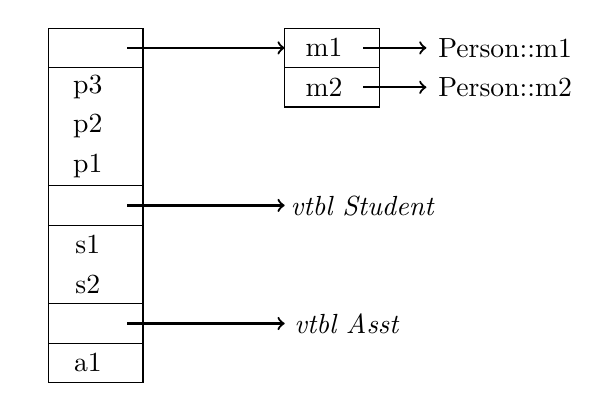
\begin{tikzpicture}

% object 3
\draw (0,-2.5)  rectangle (1.2,-3.0);
\pgftext[at={\pgfpoint{0.5cm}{-2.75cm}}]{a1} ;

% vptr object 3
\draw (0,-2.5)  rectangle (1.2,-2.0);
\pgftext[at={\pgfpoint{0.5cm}{-2.25cm}}]{} ;
\draw[->, thick] (1.0, -2.25) -- (3.0,-2.25); 
\pgftext[at={\pgfpoint{3.8cm}{-2.25cm}}]{\textit{vtbl Asst}} ;

% object 2
\draw (0,-2.0)  rectangle (1.2,-1.0);
\pgftext[at={\pgfpoint{0.5cm}{-1.25cm}}]{s1} ;
\pgftext[at={\pgfpoint{0.5cm}{-1.75cm}}]{s2} ;

% vptr
\draw (0,-1.0)  rectangle (1.2,-0.5);
\pgftext[at={\pgfpoint{-0.25cm}{-0.75cm}}]{} ;
\draw[->, thick] (1.0, -0.75) -- (3.0,-0.75); 
\pgftext[at={\pgfpoint{4.0cm}{-0.75cm}}]{\textit{vtbl Student}} ;

% object 1
\pgftext[at={\pgfpoint{0.5cm}{-0.25cm}}]{p1} ;
\pgftext[at={\pgfpoint{0.5cm}{0.25cm}}]{p2} ;
\pgftext[at={\pgfpoint{0.5cm}{0.75cm}}]{p3} ;
\draw (0,-0.5)  rectangle (1.2,1.5);

% vptr 
\draw (0,1.0)  rectangle (1.2,1.5);
\pgftext[at={\pgfpoint{0.5cm}{1.25cm}}]{} ;
\draw[->, thick] (1.0, 1.25) -- (3.0,1.25); 





% right one 

% vtbl for 

% vtbl for Person
%\draw (3,-0.5)  rectangle (4.2,0.0);
%\pgftext[at={\pgfpoint{3.5cm}{-0.25cm}}]{m4} ;
%\draw[->, thick] (4.0, -0.25) -- (4.8,-0.25); 
%\pgftext[at={\pgfpoint{5.8cm}{-0.25cm}}]{Person::m4} ;


%\draw (3,0)  rectangle (4.2,0.5);
%\pgftext[at={\pgfpoint{3.5cm}{0.25cm}}]{m3} ;
%\draw[->, thick] (4.0, 0.25) -- (4.8,0.25); 
%\pgftext[at={\pgfpoint{5.8cm}{0.25cm}}]{Person:m3} ;

\draw (3,0.5)  rectangle (4.2,1.0);
\pgftext[at={\pgfpoint{3.5cm}{0.75cm}}]{m2} ;
\draw[->, thick] (4.0, 0.75) -- (4.8,0.75); 
\pgftext[at={\pgfpoint{5.8cm}{0.75cm}}]{Person::m2} ;

\draw (3,1.0)  rectangle (4.2,1.5);
\pgftext[at={\pgfpoint{3.5cm}{1.25cm}}]{m1} ;
\draw[->, thick] (4.0, 1.25) -- (4.8,1.25); 
\pgftext[at={\pgfpoint{5.8cm}{1.25cm}}]{Person::m1} ;

\end{tikzpicture}
}
\end{tabular}

\end{tabular}

\end{frame}

\begin{frame}[fragile]
\frametitle{Name clashes (again)}
\framesubtitle{}
If two base classes define a method (field) with the same signature,
the ambiguity must be resolved. 

\begin{itemize}
\item Language-defined priorities
\begin{itemize}
\item CLOS: first-fit
\end{itemize}
\item Prohibited (and checked)
\begin{itemize}
\item Eiffel: error at compile time of the child class
\item Must be resolved manually, e.g., via \texttt{rename}; % or \texttt{select} 
\begin{eiffel}
class COURSE_ASSISTANT
inherit
      STUDENT
          rename
              name as teacher_name
          end
      PERSON
\end{eiffel}
\end{itemize}
\item Ambiguous use prohibited (and checked)
\begin{itemize}
\item \Cpp: no error at class compilation time, but at method invocation
time (statically)
\item Must be resolved manually,  via scope resolution operator
\begin{cplus3}
if (...) person::name() else student::name(); 
\end{cplus3} 
\end{itemize}
\end{itemize}
       select 
          move ..

\end{frame}


\begin{frame}[fragile]
\frametitle{Repeated inheritance}
\framesubtitle{}
In \textit{repeated}  inheritance, a class serves as 
ancestor repeatedly, through multiple inheritance relationships. 

\begin{cplus3}
class A;
class B: public A {...}
class C: public A {.. }
class D: public B, C {...}
\end{cplus3}

Replicated: 
\begin{itemize}
\item  $D$ objects contain 2 copies of $A$ objects
\item \Cpp's default choice. Shared inheritance requires keyword \texttt{virtual}.
\end{itemize}
Shared (``diamond''): 
\begin{itemize}
\item  $D$ objects contain only 1 $A$ object.
\item Eiffel's choice. Replication inheritance only via renaming. 
\end{itemize}

\end{frame}

\begin{frame}[fragile]
\frametitle{Replicated inheritance}
\framesubtitle{}
Default case in \Cpp. 
\begin{cplus3}
class A;
class B: public A {...}
class C: public A {.. }
class D: public B, C {...}
\end{cplus3}


\begin{itemize}
\item Members of $A$ are ambiguous $\leadsto$ no direct access possible
(scope resolution operator doesn't help); access via parents needed.  
\item Virtual function tables are merged  and the portions $C::A$ methods
and $B::A$ methods are kept. 

\mycomment{
\begin{cplus3}
// C++ 
A* b; B* b; C* c; D* d;
a = d; // error
b = d; 
c = d;
a = b;
a = c; 
\end{cplus3}
}
\end{itemize}
\bigskip

Problem: inconsistency
\end{frame}

\begin{frame}[fragile]
\frametitle{Shared inheritance}
\framesubtitle{}
Default case in Eiffel. In \cpp, the keyword \texttt{virtual} 
indicates sharing.
Shared inheritance avoids name clashes between parents.

\begin{cplus3}
class A;
class B: public virtual A {...}
class C: public virtual A {.. }
class D: public B, C {...}
\end{cplus3}



New ambiguity: what if both $B$ and $C$ override a method in $A$?
\begin{itemize}
\item Eiffel: use \texttt{select} to resolve ambiguity
\item \Cpp: compile-time error
\end{itemize}

General problem:


\begin{itemize}
\item In \Cpp, neither child nor virtual parent determine the construction
of parent objects---only grandchildren.
%\item In \Cpp, virtual function table gets either bigger or there is an additional level of indirection.
\item In Eiffel, it depends on the future client whether
a feature will be shared or replicated.
\end{itemize}
$\leadsto$ Implementation quite 
complicated 
\end{frame}

\begin{frame}
\frametitle{Interfaces}
\framesubtitle{}

Composing functionality is tricky, but there is not problem 
with multiple supertypes.

Via \emph{interfaces}, the programmer can define complex subtyping relations without
the problems associated with full-fledged multiple inheritance.

Example: interfaces in Java and C\#
\end{frame}


\begin{frame}[fragile]
\frametitle{Mixins}
\framesubtitle{}
\textit{Mix-in} is an alternative to full-fledged multiple inheritance which
avoids problems or complications with replicated inheritance.

\begin{itemize}
\item Same motivation: combine \textit{orthogonal} functionality
\item Group each functionality in a mix-in
\item Combining mixi
\item No superclasses: mix-in classes are in
flat hierarchies 
\item No subclasses:  a mix-in class is for
``mixing in'' properties and cannot be instantiated
\end{itemize}

Example: interfaces in Java and C\#
\end{frame}


\subsection{Binary methods}

\begin{frame}[fragile]
\frametitle{Binary methods}
\framesubtitle{Or in general: n-ary methods}
\begin{itemize}
\item Binary methods take 2 parameters of the same type.
\item 
In OOP, binary methods are methods that contain one or more parameters
of the same type as the receiver object.
\item Examples: arithmetic, equality, comparison, \ldots
\end{itemize}
\bigskip

They cause great difficulties in OOP. 
\end{frame}

\begin{frame}[fragile]
\frametitle{Binary methods problem}
\framesubtitle{Bruce, Cardelli, Hopkins Object Group }
% typing in the presence of inheritance.

Problem: 

\begin{itemize}
\item Receiver and argument are not treated symmetrically (but
should be). 
\end{itemize}


% I do not understand this...
% \bigskip

% Other problems (also big): 

% \begin{itemize}
% \item Retrofitting of new classes not possible (makes extension
% impossible)
% \item Special access rights needed (violates protection)
% %\item Do subclasses always produce subtypes?
% \end{itemize}

\end{frame}

\begin{frame}[fragile]
\frametitle{Asymmetry}
\begin{cplus3}
class Complex 
{
    // add: (Complex , Real) -> Complex  
    public Complex add(Real d) {...}
}
\end{cplus3}
How to define an addition with signature 
\begin{center}
\textit{double × Complex} → \textit{Complex}?
\end{center}
\begin{itemize}
\item Impossible in almost all OO-language (Java, C\#)!
Exception: very few (``multi-dispatch languages'') 
\item Possible in hybrid language (Ada, \Cpp) via non-OO constructs,
e.g., free functions and overloading (or ``friends''). 
\end{itemize}
\end{frame}

\begin{frame}[fragile]
\frametitle{Method dispatching}
\framesubtitle{}

Single-dispatch languages
\begin{itemize}
\item Dispatch based on the (dynamic) class of the receiver. 
\begin{cplus3}
     Complex c = ... ;   
     c.add(arg);
\end{cplus3}
\item Ex.: all languages mentioned so far

\end{itemize}

Multiple-dispatch languages
\begin{itemize}
\item Dispatch (also) based on the dynamic class of \textit{arguments}.
\item Ex.: Dylan (Apple), CLOS, Cecil
\item Deviation from previous class concept: data records + generic functions.
\begin{cplus3}
     add(arg1, arg2);
\end{cplus3}
\item Combined overloading \& overriding (resolution at run time).
\end{itemize} 
\end{frame}

\begin{frame}[fragile]
\frametitle{Multi-methods in Dylan}
\framesubtitle{}
A multi-method is a method that does not belong to one class
\begin{itemize}
\item For each binary method, there exists
a set of method bodies associated with the name of the method.
\item The dispatch depends on all parameter types.
\end{itemize}
\begin{cplus3}
// http://www.opendylan.org/books/dpg/db_88.html
// Generic ``+'' 
// Method on <time-offset>, <time-offset>
define method \+
    (offset1 :: <time-offset>, offset2 :: <time-offset>)
=> (sum :: <time-offset>)
 let sum = offset1.total-seconds + offset2.total-seconds;
 make(<time-offset>, total-seconds: sum);
end method \+;	

// Method on <time-offset>, <time-of-day>
define method \+ 
    (offset :: <time-offset>, time-of-day :: <time-of-day>)
 => (sum :: <time-of-day>)
  make(<time-of-day>, 
       total-seconds: offset.total-seconds + time-of-day.total-seconds);
end method \+;
\end{cplus3}
\end{frame}


\subsection{Overriding in real languages}

\begin{frame}[fragile]
\frametitle{Overriding rules in real languages}
\framesubtitle{}
Overriding can be \textit{covariant}, 
\textit{contravariant}, or \textit{invariant} in either
the argument types or the return type.
\bigskip


Assume a class \texttt{Animal}, a child \texttt{DomesticAnimal} with 
%a method 
%\begin{center} set_playmate(Sandwich) → void \end{center}
\begin{cplus3}
       set_playmate(DomesticAnimal)->  void 
\end{cplus3}

and the child \texttt{Cat},
which re-defines \texttt{set_playmate}. 
How may the argument type change?% (relativeto DomesticAnimal.set_playmate):
\begin{itemize}
\item Covariance (in the argument type):
\begin{cplus3}
 set_playmate(Cat) -> void
\end{cplus3}
 \item Contravariance:
\begin{cplus3}
 set_playmate(Animal) -> void
\end{cplus3}
  \item Invariance: 
\begin{cplus3}
 set_playmate(DomesticAnimal) -> void
\end{cplus3}


\end{itemize}
Eiffel uses the covariance rule; but this can be unsafe (why?).
%http://www.faqs.org/faqs/eiffel-faq/
Most languages use the invariance rule (for argument types). 
\end{frame}

\begin{frame}[fragile]
\frametitle{Covariance in return type}
\framesubtitle{}
Covariance in the return type is less contested.
\bigskip

\begin{cplus3}
// Java 1.5
class BaseClass {
    public BaseClass Clone() {..}
}
class DerivedClass extends BaseClass {
    public DerivedClass Clone() {..}
}
\end{cplus3}
Java, \Cpp, Eiffel support covariance in the return type.\\
C\# requires invariance. 
\end{frame}



\begin{frame}[fragile]
\frametitle{Pre-and postconditions in Eiffel}
\framesubtitle{Restricting replacement semantics}
\textit{Assertion redeclaration rule}: a redeclared version need not contain its own requires or ensure
clause.
\begin{itemize}
\item It may use a \texttt{require else} or
\texttt{then ensure} clause
to weaken/strengthen the pre/postcondition of the parent. 

\end{itemize}
\begin{eiffel}
class ACCOUNT 
feature
   withdraw(sum: INTEGER) is
       require
           sum >= 0
       do ..  end
end -- class ACCOUNT
class SPECIAL_ACCOUNT inherit
      ACCOUNT
      redefine withdraw end
feature
       withdraw(sum: INTEGER) is
       do ...
       ensure then
           balance >= 1000
       end
end -- class SPECIAL_ACCOUNT       
\end{eiffel}
\end{frame}



\end{document}






